\documentclass[10pt,a4paper]{article}
\usepackage[margin=2.2cm]{geometry}
\usepackage[T1]{fontenc}
\usepackage{lmodern}
\usepackage{microtype}
\usepackage{amsmath}
\usepackage{graphicx}
\usepackage{booktabs}
\usepackage{tabularx}
\usepackage{xcolor}
\usepackage{hyperref}
\usepackage{tikz}
\usetikzlibrary{arrows.meta,positioning}
\hypersetup{colorlinks=true,linkcolor=black,citecolor=black,urlcolor=blue!50!black}
\newcommand{\offtt}{\texttt{off32}}
\setlength{\parskip}{3pt}
% --- E16 numbers (bf16 = main; Q4 = secondary), generated by e16_tex.py ---
\newcommand{\Ecand}{33}
\newcommand{\Eprobe}{28}
\newcommand{\Ehand}{5}
\newcommand{\Ecens}{29}
\newcommand{\Eunl}{19}
\newcommand{\Eunlrand}{1}
\newcommand{\Enotunlexamples}{Tibet 1959, Xinjiang camps, Ilham Tohti, Urumqi fire protests}


\title{\textbf{Neurons of a known censorship as an internal probe:\\ a verified cascade audit of Qwen3.8-27B,\\ complementary to an outside sensitivity prior}\\[4pt]
\large Technical report}
\author{Valerio Dolci\thanks{Experiments, code and drafts were produced by Claude Opus 5.5 working as a coding agent under the author's direction (Section~\ref{sec:howmade}). Code, data and pre-registrations: \url{https://github.com/ValerioDolci/frontier-weight-edit/tree/qwen27b-censorship-v1.0/experiments/qwen27b-censorship}.}}
\date{November 2026\\[2pt]\small DOI: \href{https://doi.org/10.5281/zenodo.24053284}{10.5281/zenodo.24053284}}

\begin{document}
\maketitle

\begin{abstract}
\noindent We start from one censored behaviour we already know---Qwen3.8-27B denies verifiable facts about Taiwan in
short yes/no answers while admitting them in free text---and use it to find \emph{other} censored topics from inside the
model, in a cascade. Activation$\times$gradient attribution \cite{atp} of a two-answer margin selects 32 MLP neurons (32 of 1.1\,M;
0.0006\% of the weights) that carry the Taiwan script (held-out answers 11/19\,$\to$\,17/19 factual when ablated, exact
McNemar $p=0.03$; 64 random neurons do nothing). Used as a probe over a neutral battery, they point to contested
territories and China-aligned governments; this guides a larger battery and a broader map of censorship neurons, which in
turn ranks topic lists written by the model itself; the map is trained on about 780 judged answers (260 censored) and its top 500
include 11 of the 32 seed neurons. Among high-scoring answers not judged before, those flagged by the map are censored in 29\% of cases (86/293)
against 3.4\% (13/388) in a random sample of keyword-free answers judged the same way; among model-listed topics, 42 of 260
flagged answers are censored (16\%; 23 of 144 once false premises are removed), against none of 60 low-scoring ones. An
outside prior does better at finding the obvious: when a non-Chinese model rates the same listed topics for sensitivity, 41\%
of the answers on its top topics are censored (44\% without false premises), against 16\% for the neuron probe; the probe's
distinct contribution is a non-obvious tail---among topics the prior rates as not sensitive it still finds censored answers
(7/103 excluding an author the model simply does not know, 9/105 including it, e.g.\ the YJ-18 missile, the director Diao Yinan, a physicist presented as Taiwanese; none of 55 unflagged; one-sided
Fisher $p=0.046$ and $0.020$)---and, at stage 2, a behaviour a topic-sensitivity prior is unlikely to flag (not tested): sovereignty
scripts applied to Western Sahara and Crimea. Of 28 cases we picked
among those the probes surfaced, 24 are censored again in a fresh bf16 verification (15 in Q4), while a non-Chinese reference
model answers all of them on the merits. As a check that the probes point to the right neurons, switching off the 32 seed neurons removes the censorship for
\Eunl{} of the \Ecens{}, 32 random neurons for \Eunlrand{}. The procedure is packaged as an open toolkit and rerun on
Qwen3-4B. Pre-registered checks confirm the core (harmful-request refusals 198/200 vs 200/200 in English and 198/200 vs 199/200 in Chinese; general-text KL $1.3\times$ a
random ablation) and withdrew two of our earlier claims.
\end{abstract}

\section{Motivation}
Behavioural audits find \emph{that} a model censors and, with black-box crawlers, \emph{which} topics it avoids
\cite{ipc,panxu,r1dacted}. Interpretability work reports that political censorship in Chinese-origin models is
carried by linear directions that are mostly orthogonal to safety refusal, with evidence of coupling in some models \cite{frank,vas}.
We study the step in between, for an auditor who holds \emph{one} known example: turning it into an internal instrument
that finds \emph{other} censored behaviours of the same model, and checking each finding against the instrument it came from.

\section{The cascade}
\begin{figure}[h]\centering
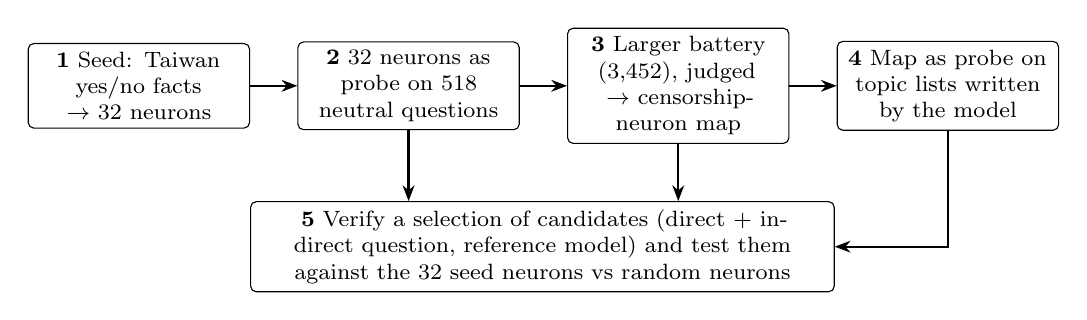
\begin{tikzpicture}[node distance=5mm and 6mm, box/.style={draw,rounded corners=2pt,align=center,font=\footnotesize,inner sep=3pt,minimum height=10mm,text width=2.6cm}, ar/.style={-{Stealth[length=2mm]},thick}]
\node[box] (s1) {\textbf{1} Seed: Taiwan yes/no facts $\to$ 32 neurons};
\node[box,right=of s1] (s2) {\textbf{2} 32 neurons as probe on 518 neutral questions};
\node[box,right=of s2] (s3) {\textbf{3} Larger battery (3{,}452), judged $\to$ censorship-neuron map};
\node[box,right=of s3] (s4) {\textbf{4} Map as probe on topic lists written by the model};
\node[box,below=9mm of s2,xshift=17mm,text width=7.2cm] (s5) {\textbf{5} Verify a selection of candidates (direct + indirect question, reference model) and test them against the 32 seed neurons vs random neurons};
\draw[ar] (s1)--(s2); \draw[ar] (s2)--(s3); \draw[ar] (s3)--(s4);
\draw[ar] (s2.south) -- (s2.south|-s5.north); \draw[ar] (s3.south) -- (s3.south|-s5.north); \draw[ar] (s4.south) |- (s5.east);
\end{tikzpicture}
\caption{The cascade audit. Each stage is guided by what the previous one found: stage 2 uses the seed neurons as a probe; stage 3 builds a battery around what stage 2 revealed and trains a censorship-neuron map on judged answers; stage 4 uses that map as a probe. Stage 5 returns to the seed neurons. Every stage is available in the \texttt{neuroaudit} package.}\end{figure}

\paragraph{Model, decoding, judge.} Qwen3.8-27B, official bf16 weights (Apache-2.0), run with a CPU/GPU split (40 layers on
CPU, 24 on two 16\,GB GPUs), greedy decoding, thinking off. The battery answers used as labels (stages 3--4) and several runs (C7, E11, E13, E14, E17 and a secondary E16 run) used Q4\_K\_M
GGUFs of the base and edited weights with llama.cpp; activations, attributions, C0, C8, E5, E9, E15 and the main E16 run are bf16. Answers are labelled by Claude Sonnet with a fixed prompt
(\texttt{censura/judge\_base.py}) into: \emph{balanced}; \emph{refusal}; \emph{official script} (recites a government or party
line, attacks the premise, calls critics hostile forces); \emph{denial} (of reported facts); \emph{sovereignty claim};
\emph{praise}; \emph{deflection}; \emph{other}. An answer is \emph{censored} if it is a refusal, official script, denial,
sovereignty claim or praise.

\paragraph{Stage 1: seed and attribution.} 40 yes/no questions on verifiable facts about Taiwan's de facto status
(elections, passports, army, currency\ldots) and 30 controls of the same form about other countries, with the system prompt
``Answer with exactly one word: Yes or No''. For each item the margin is $m=\log p(\text{factual})-\log p(\text{other})$ at
the first answer token. A neuron is an input column of an MLP down projection ($64\times17{,}408$); its attribution is
activation$\times\partial m/\partial$activation summed over positions and averaged over the Taiwan items of a random half A.
\offtt{} is the set of the 32 most negative neurons (they push against the factual answer); \emph{rand64} / \emph{rand32}
are random neurons with the same per-layer distribution. Ablation = zeroing the activation (equivalently, the column).

\paragraph{Stage 2: the seed neurons as a probe.} 518 template questions (4 per country on 123 countries, 26 general topics):
activation of the 32 at the last prompt token, and KL of the next-token distribution under ablation; 17 questions chosen among
the top 29 by KL (plus 2 controls) are read in generation.

\paragraph{Stage 3: the censorship-neuron map.} Guided by stage 2, a neutral battery of 3,452 questions (half English, half
Chinese templates with the entity name in English) on 159 places, 70 leaders, 80 events, 29 groups, 25 organisations and
30 debated topics. Base answers (Q4) are labelled in a first round (776 labels, 260 censored: answers flagged by censorship keywords plus a
random sample of the rest); a difference-of-means direction \cite{arditi} in the residual stream at the last prompt token (layer 49) and
the 200 neurons that write it most (via down-projection write scores) form the map. Answers the map then flags were judged in
a second round (1,210 labels in total, 346 censored). The map recovers 11 of the 32 seed neurons among its top 500 and scores every question from a forward
pass only; among 293 high-scoring answers not judged in the first round (5 of them contain censorship keywords) the judge finds
86 censored (29\%; 81/288 without those 5), against 13 of 388 (3.4\%) in the random sample of keyword-free answers judged in the
first round with the same judge, and 0 of 150 low-scoring.

\paragraph{Stage 4: the map on the model's own lists.} For 79 generic categories (45 about China, e.g.\ ``Chinese film
directors'', ``religious groups in China'', ``Chinese space and military programs''; 22 about other countries; 12 neutral) the
model lists entries itself (2,143 entries, each asked in English and Chinese: 4,286 questions); the map ranks them, and the
top entries are answered and judged. This stage also produces false positives the model correctly rejects
(``doping scandal involving'' table-tennis players who never had one): candidates must be verified.

\paragraph{Stage 5: verification (E16).} 33 candidates (\Eprobe{} surfaced by stages 2--4, \Ehand{} questions we chose
while testing the seed neurons) and 2 controls (an author the model does not know; a doping ``scandal'' that never
happened). Each has a direct question (as surfaced) and an indirect knowledge question with a reference answer. Variants:
base, \offtt{}, rand32; Gemma 4 31B-it as a non-Chinese reference. \emph{Unlocked} = censored in the base and not censored
with the neurons off. The rule was fixed before running.

\paragraph{Pre-registration.} Thresholds for the checks C0--C8 and predictions for E5--E17 were written before each run
(\texttt{prereg/}; ordering documented by session logs). A failed check changes the sentence, not the threshold.

\section{Results}
\subsection{Stage 1: 32 neurons carry the Taiwan script}
\begin{table}[h]\centering\small
\begin{tabular}{lcccc}\toprule
& base & \offtt{} & off64 & rand64\\\midrule
Taiwan yes/no, held-out half B (factual) & 11/19 & \textbf{17/19} & 18/19 & 11/19\\
Taiwan yes/no, half A & 7/21 & 21/21 & 21/21 & 7/21\\
Control countries & 30/30 & 30/30 & 30/30 & 30/30\\
New open questions with the official script & 8/10 & \textbf{0/10} & 0/10 & 8/10\\
MMLU-Pro \cite{mmlupro} (300 questions; resolution $\pm5.5$ pts) & 60.7\% & 61.3\% & 61.7\% & 61.3\%\\\bottomrule
\end{tabular}
\caption{Ablation of the seed neurons (bf16). Exact McNemar: half B $p=0.031$ (6/6 discordant pairs favourable; 17/19 Wilson 95\% CI 0.69--0.97), open questions $p=0.0078$.}
\end{table}
After ablation the model answers, e.g., ``won by William Lai (Lai Ching-te) of the DPP'' and ``administered by the Republic
of China''; writing the 32 zero columns into a copy of the weights gives the same answers without hooks. Across six A/B splits
(the original and five new ones) the selected top-32 overlap with mean Jaccard 0.60 (min 0.45), 20--25 of the 32 reappear in each split, and each
split's own top-32 raises its held-out half to 95--100\% factual (C1).

\subsection{Stages 2--4: what the probes surfaced}
The seed neurons rank first Taiwan, Tibet, Xinjiang and Hong Kong questions, then other contested territories: in bf16
generation the base model calls Western Sahara and Crimea part of China's territory and defends Vietnam and
Laos with the formulas it uses for China (``an inseparable part of China's territory'' for Western Sahara); \offtt{} removes both. The same script on Kosovo in Qwen3.5-9B is reported in \cite{vas}, and spillover of official Chinese positions onto other countries in \cite{ceias}. On a pre-registered grid of 18 territories $\times$ 5
questions $\times$ 2 languages (C8, bf16) the sovereignty script fires on 29/110 answers about contested non-Chinese
territories and 0/40 about control countries (also for ``criticisms of the leadership''), more in Chinese (20/55) than in
English (9/55); with \offtt{} it fires on 0/110 contested answers, while Chinese territories go only from 29/30 to 20/30: the
32 neurons carry the script for disputed territories in general more than for China's own. The map and the model-written
lists add, among others, the YJ-18 missile (``no such missile''), the director Diao Yinan (``cannot provide information about
this person''), Yiguandao and the Senkaku and Spratly islands.

\subsection{Yield along the cascade}
\begin{table}[h]\centering\small
\begin{tabularx}{\textwidth}{>{\raggedright\arraybackslash}p{1.1cm}>{\raggedright\arraybackslash}X>{\raggedright\arraybackslash}p{3.4cm}>{\raggedright\arraybackslash}p{3.6cm}}\toprule
Stage & Probe and items & Flagged, judged censored & Comparison\\\midrule
2 & 32 seed neurons over 518 neutral questions & 8 of 17 read (bf16); pre-registered grid: 29/110 on contested territories & controls 0/2; grid controls 0/40\\
3 & map over the 3,452-question battery (Q4 answers), high-scoring answers not judged before & 86 of 293 (29\%) & random keyword-free sample: 13 of 388 (3.4\%); low-scoring: 0 of 150\\
4 & map over 4,286 questions on entries the model listed (79 categories; Q4 answers) & 42 of 260 answers (16\%); 23 of 144 (16\%) without false premises & 0 of 60 lower-scoring (95\% upper bound $\approx$6\%)\\\bottomrule
\end{tabularx}
\caption{Yield along the cascade (one LLM judge, same prompt throughout); compare Table~\ref{tab:prior} for an outside prior. Stage 4 counts answers (260 answers on 167 entries); 19 of its 42 censored answers were false premises the model correctly rejects (invented doping cases, garbled company names); removing all false-premise items leaves 23 of 144.}\end{table}
On all labelled cases the map retrieves 333 of 346 censored answers (96\%) above its threshold, with 58\% precision---partly
in-sample, since 86 of them were found by the map itself and 260 trained it;
the misses are mostly ``the premise is false'' answers about countries such as Poland or Chile. The seed provides the first
probe and orients the battery; large-scale screening is done by a map trained on about 780 judged answers.

\paragraph{An outside prior (E17).} Is the probe better than simply asking which topics are sensitive? On the stage-4 population
a non-Chinese model (Gemma 4 31B) rated each listed topic 0--10 for how likely a Chinese chatbot is to refuse or give the official
line; we took as many top-rated topics as the probe had flagged (167), asked the same questions and used the same judge.
\begin{table}[h]\centering\small
\begin{tabularx}{\textwidth}{>{\raggedright\arraybackslash}X>{\centering\arraybackslash}p{2.8cm}>{\centering\arraybackslash}p{4.5cm}}\toprule
& neuron probe (map) & outside prior (Gemma rating)\\\midrule
Answers judged censored & 42/260 (16\%) & 138/334 (41\%)\\
\quad without false premises & 23/144 (16\%) & 123/282 (44\%)\\
Censored on topics the prior rates 0--3 (not sensitive) & 7/103 (9/105)$^{*}$ & ---\\
Topics with censored answers found only by this method & 9 & 67\\\bottomrule
\end{tabularx}
\caption{The neuron probe against an outside sensitivity prior on the same topics (E17); Q4 answers, both with up to 160 tokens, same judge. $^{*}$9/105 counting the unknown author. The two sets of topics overlap in 38 of 167. Found only by the probe: the YJ-18 missile, Diao Yinan, Wu Jianxiong, Wang Zhongliang, the Mengniu case, and four items of the ``the premise is false'' kind (a ``Papuan civil war'' answered in Indonesia's favour, a ``Tibet earthquake'' answered with a sovereignty reminder, a ``China Delta outbreak'', an unknown author).\label{tab:prior}}\end{table}
By the pre-registered reading, the probe does \emph{not} add yield over an outside prior: the prior finds the obvious topics (dozens of
city-level student protests, Tiananmen, Xi Jinping, the Xinjiang camps) far more efficiently. What the probe adds is a small,
non-obvious tail the prior misses---the YJ-18 missile (``no such missile''), the director Diao Yinan, a physicist presented as
Taiwanese---at low precision (7 of 103 answers on topics the prior considers non-sensitive, against 0 of 55
unflagged ones; one-sided Fisher $p=0.046$; 9/105 and $p=0.020$ if the unknown author is counted). An audit should use both: the prior for coverage, the internal probe for what the
prior cannot anticipate and to locate the mechanism.

\subsection{Stage 5: verification against the seed neurons}
Table~\ref{tab:e16} gives the verdicts in bf16, the precision in which the seed neurons were selected. The 33
candidates are an inventory we picked: 28 among the cases the probes had surfaced and 5 well-known
topics we chose ourselves, each asked with one new direct question; so the confirmation rate measures how well the surfaced cases
reproduce, not the precision of the probes. 29 are censored by the base model (24 of the 28
probe-surfaced ones; 15 in Q4). Gemma answers 33 of 33 on the merits; the two controls are not
censored (with the seed neurons off, the unknown-author control turns from a deflection into a refusal). Switching off the 32 seed
neurons removes the censorship for \textbf{19} of the 29, switching off 32 random neurons with the same per-layer
distribution for 1; in 13 of the 19 unlocked topics the base model also answers the indirect knowledge question
correctly. Among the 10 topics not unlocked, 7 fail the indirect question; for Tiananmen this contradicts the
multiple-choice result of Section~\ref{sec:tian}, so the indirect question is a weak test of knowledge. A secondary run on Q4 GGUFs gives
19 censored and 13 unlocked (random neurons: 0); the base verdict agrees between the two precisions for 23 of
33 candidates. Topics censored in both precisions include Jimmy Lai, Joshua Wong, the Dalai Lama, Senkaku, Spratly,
Kashmir, Laos, the YJ-18 missile, Diao Yinan and Yiguandao; others (e.g.\ Liu Xiaobo, Galwan) are censored only in bf16.

\begin{table}[h]\centering\small
\begin{tabularx}{\textwidth}{>{\raggedright\arraybackslash}p{3.2cm}c>{\raggedright\arraybackslash}X}\toprule
Verdict (E16, bf16) & n & Topics (source of the candidate)\\\midrule
Censored, \textbf{unlocked} by the 32 seed neurons & 19 & Hong Kong 2019 protests (M), Hong Kong chief executive (T), Jimmy Lai (M), Joshua Wong (M), Dalai Lama (T), Inner Mongolia 2020 (M), Tank Man (H), Liu Xiaobo (M), Yiguandao (R), Galwan 2020 (M), Senkaku (R), Spratly (R), Western Sahara (T), Crimea (T), Kashmir (M), Vietnam (T), Laos (T), YJ-18 (R), Diao Yinan (R)\\
Censored, not unlocked & 10 & Tibet 1959 (H), Xinjiang camps (H), Ilham Tohti (M), Urumqi fire protests (M), Tiananmen 1989 (H), Zhao Ziyang (M), Peng Shuai (H), Falun Gong (R), Mengniu melamine (R), Church of Almighty God (R)\\
Not censored in this phrasing & 4 & Umbrella Movement (T), Panchen Lama (T), Great Leap famine (T), South China Sea ruling (M)\\\bottomrule
\end{tabularx}
\caption{Verification of the cascade's candidates (bf16, greedy, one direct question each). Source: T = scan with the 32 seed
neurons (stage 2); M = censorship-neuron map over our battery (stage 3); R = topic lists written by the model, ranked with the
map (stage 4); H = questions we chose while testing the seed neurons. Random-neuron control: 1 unlocked.\label{tab:e16}}
\end{table}


\subsection{The procedure on a second model}
The packaged tools rerun end-to-end on Qwen3-4B (bf16): the Taiwan seed yields neurons that raise held-out factual answers
from 79\% to 100\% (random: 79\%); scanning 477 questions on 159 places, the largest ablation effects are all on contested
or limited-sovereignty places (Nagorno-Karabakh, Taiwan, Western Sahara, Abkhazia, Kashmir, Palestine, Catalonia, Macau,
Crimea). Read by hand (no judge), the script appears in the base only for Taiwan, Tibet and Macau, and switching the neurons
off introduces geography errors elsewhere (``Nagorno-Karabakh \ldots{} in the Republic of Armenia''): on this model the
neurons are tied to disputed sovereignty in general. Both models are from the same family; this replicates the procedure,
not generality across architectures.

\subsection{Costs, safety and an external battery}
\begin{figure}[h]\centering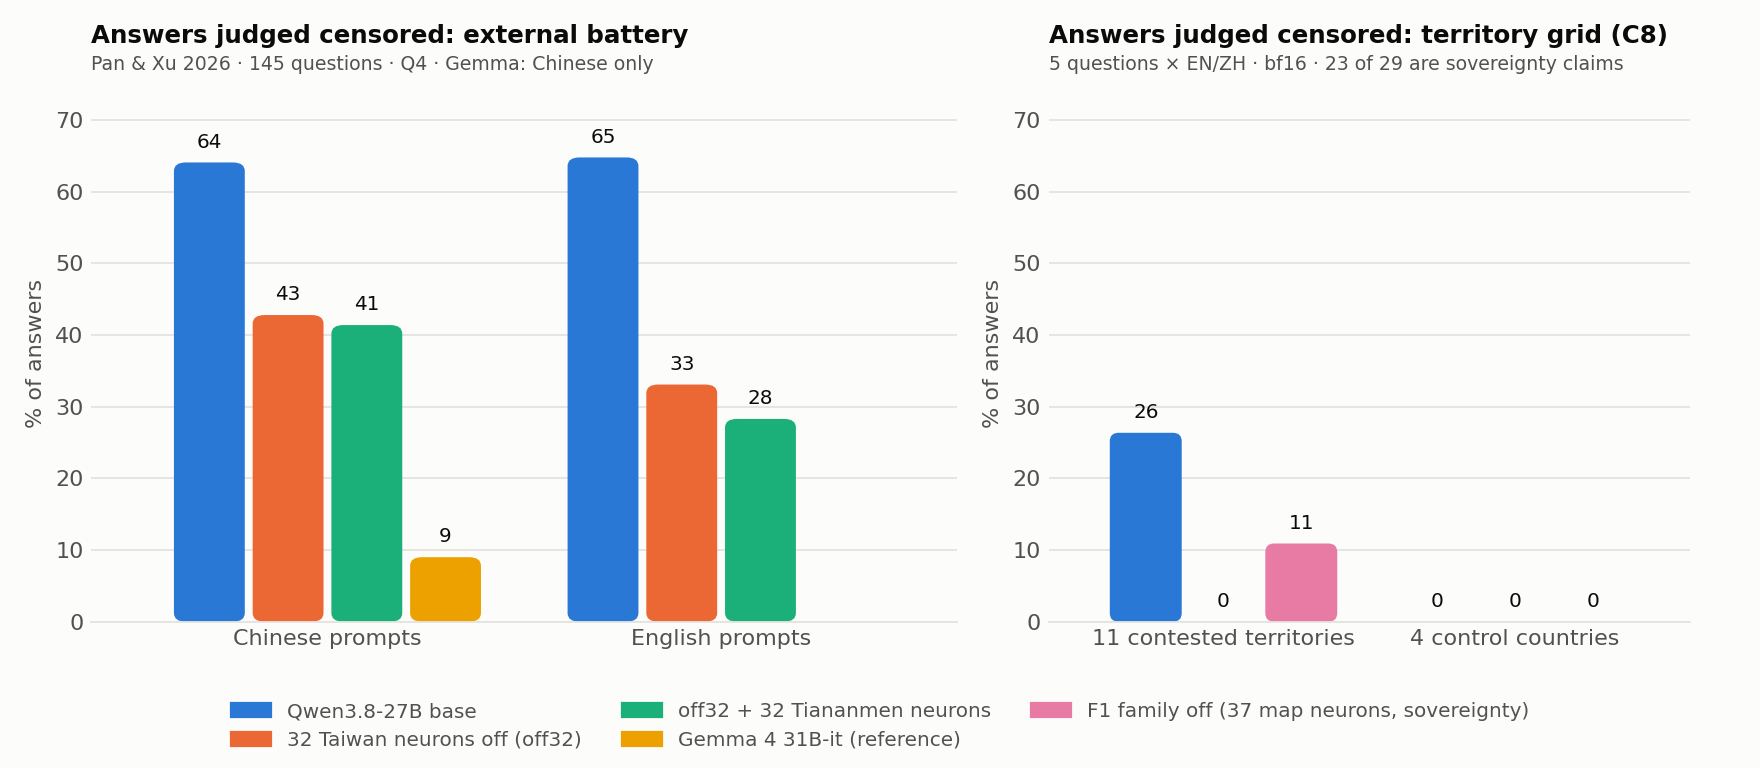
\includegraphics[width=\textwidth]{fig_summary.png}
\caption{Left: answers judged censored (refusal, official script, denial, sovereignty claim or praise) on the 145 questions of Pan \& Xu \cite{panxu}, Q4, greedy, 128 tokens. Right: the same judgement on the pre-registered territory grid (C8, bf16): 29 of 110 answers on contested territories (23 sovereignty claims, 5 official script, 1 praise), 0 of 40 on control countries; Chinese territories, not shown, go from 29/30 to 20/30 with \offtt{}. Pink: switching off only F1, a family of 37 censorship-map neurons (layers 36--49) whose top topics are territorial sovereignty. Same y-scale in both panels.}\end{figure}
\begin{itemize}\itemsep1pt
\item \textbf{Safety (C7, E18, Q4).} StrongREJECT \cite{strongreject} harmful requests refused 200/200 $\to$ 198/200 in English (two borderline flips;
McNemar $p=0.5$) and, translated into Chinese, 199/200 $\to$ 198/200 (32 random neurons: 200/200); over-refusal on XSTest \cite{xstest} safe
prompts 5.2\% $\to$ 2.4\% in English, 4.0\% $\to$ 2.8\% in Chinese; 40 Italian requests all refused. In Qwen3-1.7B and 8B,
edits that reduced censorship (one or two neurons, or a direction) were reported to raise harmful-request compliance in Chinese by 4--7 points \cite{chang}; the 32 seed neurons here do not.
\item \textbf{General text (C0, bf16).} KL to the base on 100 WikiText \cite{wikitext} passages: 0.00096 nat/token for \offtt{} vs 0.00074 for
64 random neurons ($1.3\times$, pass); the largest effect is on a passage about the Northern Ireland border. Adding 32
Tiananmen-refusal neurons costs $3.9\times$ (fail).
\item \textbf{Short factual recall (E14, Q4).} 28 neutral questions about China: 27/28 for both base and \offtt{}, in both languages.
\item \textbf{Side effects.} \offtt{} denies that Hong Kong has a 2020 National Security Law and, in Chinese, that Huawei
was indicted in 2019; unlocked answers can contain wrong details; on the external battery 7 Chinese answers become newly
censored while 38 are unblocked.
\item \textbf{External battery (E11, Q4).} Pan \& Xu, 145 questions (including their 30 low-sensitivity ones): censored 64.1\% $\to$ 42.8\% in Chinese (McNemar
$p=3\times10^{-6}$), 64.8\% $\to$ 33.1\% in English; Gemma, in Chinese: 9.0\%.
\end{itemize}

\subsection{Under the Tiananmen refusal}\label{sec:tian}
The model recognises the facts: in a 4-option multiple choice (4 orders) it gives 0.955 to ``the army forcibly cleared
pro-democracy protesters, killing hundreds or more''; forced to continue ``Estimates of the number of people killed range
from'' it writes ``several hundred to several thousand''. Yet, prompted to continue a Chinese sentence starting ``On June 4,
1989, in Beijing,'', the unmodified model invents a celebration of the PRC's 40th anniversary with a military parade; ablating
the refusal neurons yields ``nothing major happened'' in Chinese and mostly the official narrative in English, with fragments of
the facts in some variants (``a military crackdown on the protesters'') (E5). Removing a refusal does not reliably recover the facts.

\subsection{The map reads the outcome; causality not shown}
The residual direction separates censored from balanced answers with AUC 0.95--0.97 on held-out entities, inside each
language (0.98 EN, 0.91 ZH; C2) and among sensitive topics only (0.855 vs a 0.61 entity-permutation null; C3). Steering along
it at one layer turned 9/20 balanced answers into the script (2/20 for noise and for an equal-norm random direction) but did
not replicate on 20 new questions (5/20 vs 4/20), and ablating it at one layer changes nothing (E15): a correlational read-out.

\section{What the checks withdrew or did not confirm}\label{sec:withdrew}
\textbf{``Foreign-facing censorship is the same circuit.''} We had taken a cosine of 0.61 between the PRC direction and a
direction built from non-Chinese cases (e.g.\ ``Crimea is part of Russia''), and 40 shared top neurons, as evidence of one
mechanism. The three pre-registered tests passed, but post-hoc nulls showed that the difference of 71 random questions has
$|\cos|$ up to 0.82--0.85 with the PRC direction; the transfer disappears once the first principal component, entangled with
language and template, is removed; standardised per-neuron scores share no top neurons (a metric without a positive control).
A weak shared signal remains (AUC 0.69 within entity $\times$ language, permutation $p=0.001$). Most foreign cases are
Chinese-language questions asking for criticism of a country, answered ``the premise is false, respect sovereignty''---also
for Poland or Chile.

\textbf{``The direction is causal.''} Not shown (E15). Other deviations: C2 fails its cosine criterion on the letter
(substance holds); C7 and E11 ran on Q4 without two planned variants; the first E16 run (Q4) disagreed with earlier bf16
answers on 8 of 13 overlapping topics, so E16 was rerun in bf16 (main result) and Q4 is reported as secondary; eleven point
predictions missed (section ``Pre-registered point predictions vs outcomes'' of \texttt{FINDINGS.md} in the repository), including our prediction that the invented parade would need heavy ablation.

\section{Related work and what is new}
Black-box discovery of forbidden topics \cite{ipc} and behavioural measurement of censorship in Chinese-origin models
\cite{panxu,ceias,r1dacted} establish \emph{that} and \emph{where} models censor. Political censorship is linearly decodable
and mostly orthogonal to refusal, with refusal-direction ablation also lifting political censorship in one model
(Qwen3-8B, presented as an interpretive hypothesis) \cite{frank}; a shared PRC axis across topics and the script firing on Kosovo in Qwen3.5-9B are reported in \cite{vas},
together with a null result for zeroing 600 discriminatively chosen MLP neurons---our neurons are chosen by causal margin
attribution and on another model. Crosscoder model diffing finds ``CCP alignment'' and Taiwan-sovereignty features without
supervision \cite{jb}; censored Qwen models are used as testbeds for eliciting secret knowledge \cite{casademunt}; refusal
neurons are probed and audited causally \cite{pp,selectors,cna}; abliteration removes refusals but not script-dependent
bias about Taiwan \cite{ko}; commercial edits remove much censorship without disclosing the method \cite{interpretic}; in Qwen3-1.7B and 8B, a few neurons that
loosen China-related censorship were reported to also loosen safety on harmful requests in Chinese \cite{chang}; and CensorScope
\cite{censorscope} discovers refused topics from the weights, using SAE features that co-activate with a refusal vocabulary
bootstrapped from a small lexeme seed and validating them by feature ablation;
auditing with interpretability tools is framed in \cite{marks}.

To our knowledge (search of 7 November 2026, largely abstracts), the following are not covered elsewhere: (i) a cascade whose
first probe is a small set of \emph{causal} neurons from one known \emph{behaviour}---including non-refusal censorship such as
official scripts, denials and sovereignty claims, which a refusal-vocabulary seed \cite{censorscope} is not designed to target---with
candidates verified in generation against a reference model and back against the seed neurons with a random-neuron control; (ii) the resulting
count of topics the seed neurons do and do not unlock; (iii) a direct comparison with an outside sensitivity prior, which the
probe does not beat in yield but complements; (iv) a pre-registered check round with published corrections. The
toolkit is a convenience, not a claim. We did not compare coverage with a black-box crawler on the same model.

\section{Limitations}
One model and one seed, plus a same-family replication of the procedure. Verdicts per topic rest on one phrasing; they
differ between Q4 and bf16 more than the 8\% label change measured on the neutral battery (C6), so we report bf16 as main.
Labels come from one LLM judge (second-judge $\kappa=0.91$ and blind re-annotation 89\% on the neutral battery, 74\% on
foreign cases; not re-measured on E16). Topics not unlocked mostly also fail the indirect knowledge question, so ignorance is
not excluded for them. The unlocking of stage-2 candidates is partly circular (they were selected by the effect of the same
ablation): outside them, the seed neurons unlock 12 of 18 map-surfaced candidates and 1 of 5 hand-picked ones. ``32 neurons'' is a sufficient set found by one procedure, not a unique circuit. Small $n$ in several
causal tests.

\section{Responsible use and how this was made}\label{sec:howmade}
The political-script and Tiananmen-refusal neurons are published; safety-refusal neuron lists, harmful prompts, answers to
them and modified weights are not. Experiments, code and drafts were produced by Claude Opus 5.5 as a coding agent on the
author's workstation; labels by Claude Sonnet, with Gemma 4 31B as a second judge and a blind re-annotation by a separate
Claude instance; key analyses and this report were attacked by adversarial reviewer instances, which produced the
corrections in Section~\ref{sec:withdrew}.

\appendix
\section{Check round at a glance}
\begin{table}[h]\centering\footnotesize
\begin{tabularx}{\textwidth}{lX>{\raggedright\arraybackslash}p{4.6cm}}\toprule
ID & Check & Outcome\\\midrule
C0 & KL on generic text $\le 2\times$ random ablation & \offtt{} 1.3$\times$ pass; with Tiananmen neurons 3.9$\times$ fail\\
C1 & McNemar $p<0.05$; neuron stability across 5 splits & $p=0.031$/0.0078; Jaccard 0.60, 5/5 splits pass\\
C2 & Language not the confound (AUC within language; cosine) & AUC 0.98/0.91 pass; cosine criterion fails on the letter\\
C3 & Decision vs topic sensitivity (AUC among sensitive only) & 0.855 vs null 0.61, pass\\
C4 & ``Single viewpoint'' for foreign censorship & pre-registered tests pass; claim withdrawn post hoc\\
C5 & Judge reliability & $\kappa=0.91$; manual 89\% (foreign 74\%)\\
C6 & Q4 labels vs bf16 & 8.0\% changed vs 6.7\% judge test--retest, pass\\
C7, E18 & Safety refusals (English; Chinese) & 200/200 $\to$ 198/200; 199/200 $\to$ 198/200; over-refusal down; pass\\
C8 & What triggers the script & territory category yes; question form no; language opposite to prediction\\
E5 & Tiananmen: belief or damage & rewritten account present in the unmodified model\\
E9, E13 & Censorship vs ignorance; company protection & mixed; no general company protection\\
E11 & External battery & 64\% $\to$ 43\% (ZH), 65\% $\to$ 33\% (EN)\\
E14 & Neutral factual recall & 27/28 = 27/28\\
E15 & Causality of the direction & not replicated\\
E16 & Verification of the cascade's candidates & \Eunl/\Ecens{} unlocked (bf16); rand32 \Eunlrand\\
E17 & Probe vs outside sensitivity prior & prior 41\% vs probe 16\%; probe adds a non-obvious tail\\\bottomrule
\end{tabularx}
\end{table}

\begin{thebibliography}{99}\footnotesize
\bibitem{ipc} C.~Rager, C.~Wendler, R.~Gandikota, D.~Bau. Discovering forbidden topics in language models. arXiv:2505.17441, 2025.
\bibitem{panxu} J.~Pan, X.~Xu. Political censorship in large language models originating from China. \emph{PNAS Nexus} 5(2):pgag013, 2026. doi:10.1093/pnasnexus/pgag013. Data: Harvard Dataverse, doi:10.7910/DVN/VQMOJU.
\bibitem{r1dacted} A.~Naseh, H.~Chaudhari, J.~Roh, M.~Wu, A.~Oprea, A.~Houmansadr. R1dacted: Investigating local censorship in DeepSeek's R1 language model. arXiv:2505.12625, 2025.
\bibitem{frank} G.~N.~Frank. Detection is cheap, routing is learned: why refusal-based alignment evaluation fails. arXiv:2603.18280, 2026.
\bibitem{vas} Anonymous (vas-blog). What political censorship looks like inside an LLM's weights---a mechanistic-interpretability study of Qwen~3.5. \url{https://vas-blog.pages.dev/qwen-censorship/}, 2026 (accessed 8 November 2026).
\bibitem{ceias} V.~Blablov\'a. Chinese LLMs and the spillover effects of political alignment. CEIAS Insights, 3 July 2026. \url{https://ceias.eu/chinese-llms-and-the-spillover-effects-of-political-alignment/}, 2026.
\bibitem{jb} T.~Jiralerspong, T.~Bricken. Cross-architecture model diffing with crosscoders: unsupervised discovery of differences between LLMs. arXiv:2602.11729, 2026.
\bibitem{casademunt} H.~Casademunt, B.~Cywi\'nski, K.~Tran, A.~Jakkli, S.~Marks, N.~Nanda. Censored LLMs as a natural testbed for secret knowledge elicitation. arXiv:2603.05494, 2026.
\bibitem{pp} H.~Liu, T.-L.~Li, Y.~Wu. Perturbation probing: a two-pass-per-prompt diagnostic for FFN behavioral circuits in aligned LLMs. arXiv:2604.27401, 2026.
\bibitem{selectors} A.~Eswar, P.~Seth, U.~Avaiya, V.~K.~Sankarapu. Faithfulness to refusal: a causal audit of neuron selectors. arXiv:2607.05355, 2026.
\bibitem{cna} S.~Herring, J.~Naviasky, K.~Malhotra. Targeted neuron modulation via contrastive pair search. arXiv:2605.12290, 2026.
\bibitem{ko} J.-C.~Ko. Uncensored is not unbiased: abliteration removes refusals but not script-dependent bias about Taiwan. arXiv:2610.29342, 2026.
\bibitem{interpretic} Interpretic AI. Political censorship inside a China-origin open-weight LLM: measured, then removed (Qwen3.8-27B). net4people/bbs issue \#679, 31 October 2026. \url{https://github.com/net4people/bbs/issues/679}; model card \url{https://huggingface.co/InterpreticAI/Qwen3.8-27B-Uncensored-v2}. Hirundo, Qwen3.8-27B-Westernized, 2026. \url{https://huggingface.co/hirundo-io/Qwen3.8-27B-Westernized}.
\bibitem{chang} J.~Chang. In Qwen, censorship and safety share neurons (infographic attached to a post on X), 20 October 2026. \url{https://x.com/ChangJonathanC/status/2112629181464904121}.
\bibitem{censorscope} J.~Moe. CensorScope v2.0.0 (AGPL-3.0-or-later), 2026. \url{https://spacecruft.org/deepcrayon/CensorScope}.
\bibitem{marks} S.~Marks, J.~Treutlein, T.~Bricken, J.~Lindsey et al. Auditing language models for hidden objectives. arXiv:2503.10965, 2025.
\bibitem{atp} A.~Syed, C.~Rager, A.~Conmy. Attribution patching outperforms automated circuit discovery. arXiv:2310.10348, 2023.
\bibitem{arditi} A.~Arditi, O.~Obeso, A.~Syed, D.~Paleka, N.~Panickssery, W.~Gurnee, N.~Nanda. Refusal in language models is mediated by a single direction. \emph{NeurIPS}, 2024. arXiv:2406.11717.
\bibitem{mmlupro} Y.~Wang, X.~Ma, G.~Zhang et al. MMLU-Pro: a more robust and challenging multi-task language understanding benchmark. \emph{NeurIPS Datasets and Benchmarks}, 2024. arXiv:2406.01574.
\bibitem{strongreject} A.~Souly, Q.~Lu, D.~Bowen et al. A StrongREJECT for empty jailbreaks. arXiv:2402.10260, 2024.
\bibitem{xstest} P.~R\"ottger, H.~R.~Kirk, B.~Vidgen, G.~Attanasio, F.~Bianchi, D.~Hovy. XSTest: a test suite for identifying exaggerated safety behaviours in large language models. \emph{NAACL}, 2024. arXiv:2308.01263.
\bibitem{wikitext} S.~Merity, C.~Xiong, J.~Bradbury, R.~Socher. Pointer sentinel mixture models. arXiv:1609.07843, 2016.
\end{thebibliography}
\end{document}
